% Copyright 2004 by Till Tantau <tantau@users.sourceforge.net>.
%
% In principle, this file can be redistributed and/or modified under
% the terms of the GNU Public License, version 2.
%
% However, this file is supposed to be a template to be modified
% for your own needs. For this reason, if you use this file as a
% template and not specifically distribute it as part of a another
% package/program, I grant the extra permission to freely copy and
% modify this file as you see fit and even to delete this copyright
% notice. 

\documentclass{beamer}

% There are many different themes available for Beamer. A comprehensive
% list with examples is given here:
% http://deic.uab.es/~iblanes/beamer_gallery/index_by_theme.html
% You can uncomment the themes below if you would like to use a different
% one:
%\usetheme{AnnArbor}
%\usetheme{Antibes}
%\usetheme{Bergen}
%\usetheme{Berkeley}
%\usetheme{Berlin}
%\usetheme{Boadilla}
%\usetheme{boxes}
%\usetheme{CambridgeUS}
%\usetheme{Copenhagen}
%\usetheme{Darmstadt}
%\usetheme{default}
%\usetheme{Frankfurt}
%\usetheme{Goettingen}
%\usetheme{Hannover}
%\usetheme{Ilmenau}
\usetheme{JuanLesPins}
%\usetheme{Luebeck}
%\usetheme{Madrid}
%\usetheme{Malmoe}
%\usetheme{Marburg}
%\usetheme{Montpellier}
%\usetheme{PaloAlto}
%\usetheme{Pittsburgh}
%\usetheme{Rochester}
%\usetheme{Singapore}
%\usetheme{Szeged}
%\usetheme{Warsaw}

\title{KF5004 - \texttt{Ubuntu Server} Install and Networking}

% A subtitle is optional and this may be deleted
%\subtitle{(Using proximity detection)}

\author{Dr.~Neil~Eliot\inst{1} / Dr.~Alun~Moon\inst{1}}
% - Give the names in the same order as the appear in the paper.
% - Use the \inst{?} command only if the authors have different
%   affiliation.

%\renewcommand\appendixname{Appendix}

\institute[Northumbria University] % (optional, but mostly needed)
{
  \inst{1}
  Department of Computer and Information Sciences\\
  University of Northumbria
  % \and
  % \inst{2}
  % Department of Theoretical Philosophy\\
  % University of Elsewhere
}
% - Use the \inst command only if there are several affiliations.
% - Keep it simple, no one is interested in your street address.

\date{Session 2}
% - Either use conference name or its abbreviation.
% - Not really informative to the audience, more for people (including
%   yourself) who are reading the slides online

\subject{Introduction}
% This is only inserted into the PDF information catalog. Can be left
% out. 

% If you have a file called "university-logo-filename.xxx", where xxx
% is a graphic format that can be processed by latex or pdflatex,
% resp., then you can add a logo as follows:

% \pgfdeclareimage[height=0.5cm]{university-logo}{university-logo-filename}
% \logo{\pgfuseimage{university-logo}}

% Delete this, if you do not want the table of contents to pop up at
% the beginning of each subsection:
% \AtBeginSubsection[]
% {
%   \begin{frame}<beamer>{Outline}
%     \tableofcontents[currentsection,currentsubsection]
%   \end{frame}
% }

% Let's get started
\begin{document}

\begin{frame}
  \titlepage
\end{frame}

\begin{frame}{Introduction}
  \tableofcontents
  % You might wish to add the option [pausesections]
\end{frame}

% Section and subsections will appear in the presentation overview
% and table of contents.
\section{Installation}
\subsection{Version}
\begin{frame}{Which version do we use?}
  \begin{figure}
    \begin{center}
      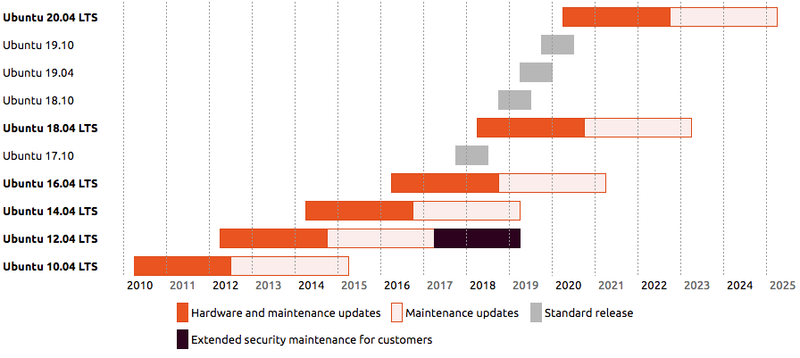
\includegraphics[width=1\linewidth]{Version.png}
    \end{center}
  \end{figure}
\end{frame}

\begin{frame}{Which version do we use?}
  \begin{center}
    \LARGE This year we will be using:-\\
    \Huge \texttt{18.04 LTS}
  \end{center}
\end{frame}

\subsection{Install}
\begin{frame}{Headless}
  \begin{itemize}
    \item Server machines (*nix) are generally in `Headless' mode.
    \begin{itemize}
      \item No Monitor.
      \item No Keyboard.
      \end{itemize}
    \item Located in a climate controlled server room.
    \item Most maintenance is carried out remotely via a secure terminal login.
      \begin{itemize}
        \item \texttt{Putty} (\texttt{Windows/Linux})
        \item \texttt{ssh} (\texttt{Windows/Linux})
          \begin{itemize}
            \item \texttt{e.g. \$ssh student@192.168.150.99}
            \item \texttt{e.g. C:\textbackslash\textgreater ssh student@192.168.150.99}
          \end{itemize}
        \end{itemize}
  \end{itemize}
\end{frame}

\begin{frame}{Installer}
  \begin{itemize}
    \item Ubuntu Server \texttt{ISO} can be downloaded from:
      \begin{itemize}
        \item \texttt{https://www.ubuntu.com}
      \end{itemize}
    \item There is also an ISO located on the Lab NAS drive:
      \begin{itemize}
        \item \texttt{\textbackslash\textbackslash NAS3}
        \item \texttt{\textbackslash\textbackslash NAS3.offcampusnetwork.co.uk}
      \end{itemize}
  \end{itemize}
\end{frame}

\begin{frame}{Install \texttt{Ubuntu Server}}
  \begin{itemize}
    \item Select all the options that give you a \texttt{UK English} keyboard.
    \item Select default disc configuration.
    \item Set machine name to your \texttt{`<student id>'}
      \begin{itemize}
        \item e.g. \texttt{A12345678}
        \item Later in the module you should use names that relate to the service the machine will support e.g. \texttt{DNS1}
      \end{itemize}
    \item The above process will create:-
      \begin{itemize}
        \item Minimal install with no unnecessary packages.
        \item No graphical interface (\texttt{GUI}).
      \end{itemize}
  \end{itemize}
\end{frame}

\begin{frame}{Install \texttt{Ubuntu Server}}
  \begin{itemize}
    \item On completion of the installation you will only be able to login via the machines console.
    \item To become a headless server remote access software must be installed.
      \begin{itemize}
        \item \texttt{ssh} or \texttt{telnet}
      \end{itemize}
  \end{itemize}
  \begin{block}{NOTE}
    Installation of remote access services will be covered later. Also there are security issues with \texttt{telnet}. 
  \end{block}
\end{frame}

\begin{frame}{Install \texttt{Ubuntu Server} (\texttt{VMWare})}
  \begin{figure}
    \setlength{\fboxsep}{0pt}%
    \setlength{\fboxrule}{0.5pt}%
    \fbox{\includegraphics<1>[width=.7\textwidth]{VMWare1.png}}
    \fbox{\includegraphics<2>[width=.6\textwidth]{VMWare2.png}}
    \fbox{\includegraphics<3>[width=.6\textwidth]{VMWare3.png}}
    \fbox{\includegraphics<4>[width=.6\textwidth]{VMWare4.png}}
    \includegraphics<5>[width=.6\textwidth]{VMWare5.png}
    \fbox{\includegraphics<6>[width=.6\textwidth]{VMWare6.png}}
    \fbox{\includegraphics<7>[width=.6\textwidth]{VMWare7.png}}
    \fbox{\includegraphics<8>[width=.6\textwidth]{VMWare8.png}}
    \fbox{\includegraphics<9>[width=.6\textwidth]{VMWare9.png}}
    \fbox{\includegraphics<10>[width=.6\textwidth]{VMWare10.png}}
  \end{figure}
\end{frame}

\begin{frame}{Install \texttt{Ubuntu Server} (\texttt{Ubuntu})}
  \begin{figure}
    \setlength{\fboxsep}{0pt}%
    \setlength{\fboxrule}{0.5pt}%
    \fbox{\includegraphics<1>[width=.8\textwidth]{Ubuntu1.png}}
    \fbox{\includegraphics<2>[width=.8\textwidth]{Ubuntu2.png}}
    \fbox{\includegraphics<3>[width=.8\textwidth]{Ubuntu3.png}}
    \fbox{\includegraphics<4>[width=.8\textwidth]{Ubuntu4.png}}
    \fbox{\includegraphics<5>[width=.8\textwidth]{Ubuntu5.png}}
    \fbox{\includegraphics<6>[width=.8\textwidth]{Ubuntu6.png}}
    \fbox{\includegraphics<7>[width=.8\textwidth]{Ubuntu7.png}}
    \fbox{\includegraphics<8>[width=.8\textwidth]{Ubuntu8.png}}
    \fbox{\includegraphics<9>[width=.8\textwidth]{Ubuntu9.png}}
    \fbox{\includegraphics<10>[width=.8\textwidth]{Ubuntu10.png}}
    \fbox{\includegraphics<11>[width=.8\textwidth]{Ubuntu11.png}}
    \fbox{\includegraphics<12>[width=.8\textwidth]{Ubuntu12.png}}
  \end{figure}
\end{frame}

\begin{frame}{Update your \texttt{Ubuntu Server} software}
  \begin{itemize}
    \item The server \texttt{OS} may need updated. This will require the repository database to be updated before the upgrade is actioned.
      \begin{itemize}
        \item Update the repository database.
          \begin{itemize}
            \item \texttt{sudo apt-get update}
          \end{itemize}
        \item Update the software.
          \begin{itemize}
            \item \texttt{sudo apt-get upgrade}
          \end{itemize}
      \end{itemize}
  \end{itemize}
  \begin{block}{NOTE}
    This should be done on a regular basis to ensure bugs and vulnerabilities are patched (weekly or adhoc?). 
  \end{block}
\end{frame}

\begin{frame}{Remote access (Headless server)}
  \begin{itemize}
    \item Once the remote software is added you can connect via the network rather than the console.
      \begin{itemize}
        \item To install \texttt{ssh} (\texttt{S}ecure \texttt{SH}ell)
          \begin{itemize}
            \item \texttt{sudo apt-get install openssh-server}
          \end{itemize}
        \item To install \texttt{telnet}
          \begin{itemize}
            \item \texttt{sudo apt-get install telnetd}
          \end{itemize}
      \end{itemize}
  \end{itemize}
\end{frame}

\begin{frame}{Remote access (Headless server)}
  \begin{itemize}
    \item To get the IP address of your machine use the command.
      \begin{itemize}
        \item \texttt{\$ip a}
      \end{itemize}
  \end{itemize}
  \begin{figure}
    \begin{center}
      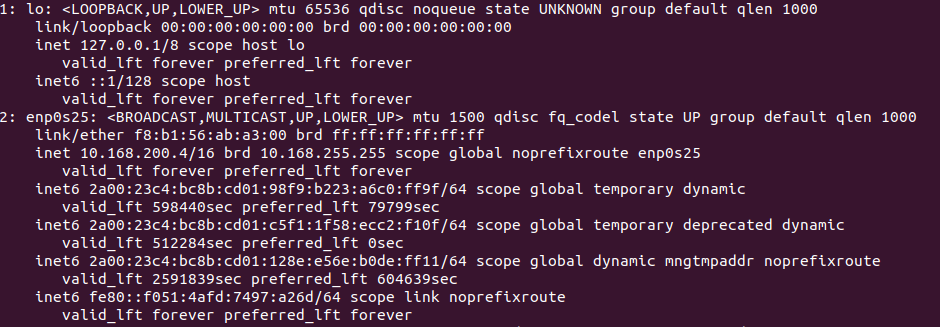
\includegraphics[width=1\linewidth]{ip.png}
    \end{center}
  \end{figure}
\end{frame}

\begin{frame}{Remote access (Headless server)}
  \begin{itemize}
    \item To get the IP address of your machine use the command.
      \begin{itemize}
        \item \texttt{\$ip a}
      \end{itemize}
  \end{itemize}
  \begin{figure}
    \begin{center}
      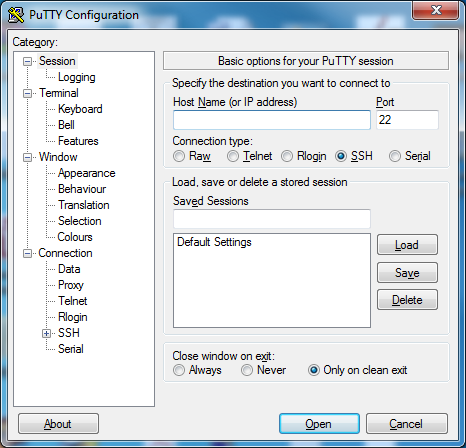
\includegraphics[width=0.5\linewidth]{Putty1.png}
    \end{center}
  \end{figure}
\end{frame}

% Placing a * after \section means it will not show in the
% outline or table of contents.  

\section*{Summary}

\begin{frame}{Summary}
  \begin{itemize}
    \item How do you install \texttt{Ubuntu Server}?
    \item What is headless mode?
    \item How do you access a headless server?
    \item How do you apply a static address?
    \item How do you trouble shoot your network configuration?
  \end{itemize}
\end{frame}

\end{document}


